% !TeX spellcheck = en_US
% !TeX encoding = UTF-8
% !TeX root = thesis.tex

% ******************************* PhD Thesis Template **************************
% Please have a look at the README.md file for info on how to use the template

\documentclass[a4paper,12pt,times,print,withindex,twoside,custommargin]{PhDThesisPSnPDF}

% ******************************************************************************
% ******************************* Class Options ********************************
% *********************** See README for more details **************************
% ******************************************************************************

% `a4paper'(The University of Cambridge PhD thesis guidelines recommends a page
% size a4 - default option) or `a5paper': A5 Paper size is also allowed as per
% the Cambridge University Engineering Deparment guidelines for PhD thesis
%
% `11pt' or `12pt'(default): Font Size 10pt is NOT recommended by the University
% guidelines
%
% `oneside' or `twoside'(default): Printing double side (twoside) or single
% side.
%
% `print': Use `print' for print version with appropriate margins and page
% layout. Leaving the options field blank will activate Online version.
%
% `withindex': For index at the end of the thesis
%
% `draftclassic': For draft mode without loading any images (same as draft in book)
%
% `draft': Special draft mode with line numbers, images, and water mark with
% timestamp and custom text. Position of the text can also be modified.
%
% `abstract': To generate only the title page and abstract page with
% dissertation title and name, to submit to the Student Registry
%
% `chapter`: This option enables only the specified chapter and it's references
%  Useful for review and corrections.
%
% ************************* Custom Page Margins ********************************
%
% `custommargin`: Use `custommargin' in options to activate custom page margins,
% which can be defined in the preamble.tex. Custom margin will override
% print/online margin setup.
%
% *********************** Choosing the Fonts in Class Options ******************
%
% `times' : Times font with math support. (The Cambridge University guidelines
% recommend using times)
%
% `fourier': Utopia Font with Fourier Math font (Font has to be installed)
%            It's a free font.
%
% `customfont': Use `customfont' option in the document class and load the
% package in the preamble.tex
%
% default or leave empty: `Latin Modern' font will be loaded.
%
% **************************** Choosing the Page Style *************************
%
% `default (leave empty)': For Page Numbers in Header (Left Even, Right Odd) and
% Chapter Name in Header (Right Even) and Section Name (Left Odd). Blank Footer.
%
% `PageStyleI': Chapter Name next & Page Number on Even Side (Left Even).
% Section Name & Page Number in Header on Odd Side (Right Odd). Footer is empty.
%
% `PageStyleII': Chapter Name on Even Side (Left Even) in Header. Section Number
% and Section Name in Header on Odd Side (Right Odd). Page numbering in footer

% ********************************** Preamble **********************************
% Preamble: Contains packages and user-defined commands and settings
% ******************************************************************************
% ****************************** Custom Margin *********************************

% Add `custommargin' in the document class options to use this section
% Set {innerside margin / outerside margin / topmargin / bottom margin}  and
% other page dimensions
\ifsetCustomMargin
  \RequirePackage[left=25mm,right=25mm,top=29mm,bottom=25mm]{geometry}
  %\RequirePackage[left=37mm,right=30mm,top=35mm,bottom=30mm]{geometry}
  \setFancyHdr % To apply fancy header after geometry package is loaded
\fi

% Add spaces between paragraphs
%\setlength{\parskip}{0.5em}
% Ragged bottom avoids extra whitespaces between paragraphs
% \raggedbottom
% To remove the excess top spacing for enumeration, list and description
%\usepackage{enumitem}
%\setlist[enumerate,itemize,description]{topsep=0em}

% *****************************************************************************
% ******************* Fonts (like different typewriter fonts etc.)*************

% Add `customfont' in the document class option to use this section

\ifsetCustomFont
  % Set your custom font here and use `customfont' in options. Leave empty to
  % load computer modern font (default LaTeX font).
  %\RequirePackage{helvet}

  % For use with XeLaTeX
  %  \setmainfont[
  %    Path              = ./libertine/opentype/,
  %    Extension         = .otf,
  %    UprightFont = LinLibertine_R,
  %    BoldFont = LinLibertine_RZ, % Linux Libertine O Regular Semibold
  %    ItalicFont = LinLibertine_RI,
  %    BoldItalicFont = LinLibertine_RZI, % Linux Libertine O Regular Semibold Italic
  %  ]
  %  {libertine}
  %  % load font from system font
  %  \newfontfamily\libertinesystemfont{Linux Libertine O}
\fi

% *****************************************************************************
% **************************** Custom Packages ********************************

% ************************* My Custom Packages *********************************
\usepackage[a-2b]{pdfx}
\usepackage[export]{adjustbox}
\usepackage{color, colortbl}
\usepackage{enumitem}
\usepackage{tcolorbox}
\usepackage{setspace}
\usepackage[nopostdot,nonumberlist,acronym,toc]{glossaries}
\usepackage{xurl}
\usepackage[fontsize=13]{fontsize}
\usepackage{caption}
\usepackage{listings}
\usepackage{mathpartir}
\usepackage{newfloat}
\usepackage{overpic}
\usepackage{rotating}
\usepackage{tikz}
\usetikzlibrary{shapes,arrows.meta,positioning,fit,calc,tikzmark}
\usepackage{tipa}
\captionsetup[table]{font={stretch=1.3},labelfont=bf}     %% change 1.2 as you like
\captionsetup[figure]{font={stretch=1.3}, labelfont=bf}
\usepackage[normalem]{ulem}
\newcommand{\stkout}[1]{\ifmmode\text{\sout{\ensuremath{#1}}}\else\sout{#1}\fi}

% ************************* Algorithms and Pseudocode **************************

\usepackage{algorithm}
\usepackage[noend]{algpseudocode}

% knuth style line numbers (3.5 instead of 5)
\algrenewcommand{\alglinenumber}[1]{\makebox[2.5em]{\thealgorithm.#1}}
\makeatletter 
\renewcommand\thealgorithm{\thechapter.\arabic{algorithm}} 
\@addtoreset{algorithm}{chapter} 
\makeatother


% ******************************** Math Stuff **********************************

\usepackage{amsthm}
\theoremstyle{definition}
\newtheorem{definition}{Definition}[chapter]
\newtheorem{theorem}{Theorem}[chapter]

% ********************Captions and Hyperreferencing / URL **********************

% Captions: This makes captions of figures use a boldfaced small font.
%\RequirePackage[small,bf]{caption}


% *************************** Graphics and figures *****************************

%\usepackage{rotating}
%\usepackage{wrapfig}

% Uncomment the following two lines to force Latex to place the figure.
% Use [H] when including graphics. Note 'H' instead of 'h'
%\usepackage{float}
%\restylefloat{figure}

% Subcaption package is also available in the sty folder you can use that by
% uncommenting the following line
% This is for people stuck with older versions of texlive
%\usepackage{sty/caption/subcaption}
\usepackage{subcaption}

% ********************************** Tables ************************************
\usepackage{booktabs} % For professional looking tables
\usepackage{multirow}
\usepackage{multicol}
\usepackage{lipsum} 
%\usepackage{longtable}
%\usepackage{tabularx}


% *********************************** SI Units *********************************
\usepackage{siunitx} % use this package module for SI units


% ******************************* Line Spacing *********************************

% Choose linespacing as appropriate. Default is one-half line spacing as per the
% University guidelines

% \doublespacing
% \onehalfspacing
% \singlespacing
\setstretch{1.3} % 1.4 or 1.3 as per HSG printing guidelines


% ************************ Formatting / Footnote *******************************

% Don't break enumeration (etc.) across pages in an ugly manner (default 10000)
%\clubpenalty=500
%\widowpenalty=500

%\usepackage[perpage]{footmisc} %Range of footnote options


% *****************************************************************************
% *************************** Bibliography  and References ********************

\usepackage{cleveref} %Referencing without need to explicitly state fig /table


\makeatletter
% Named labels: First argument is reference, second is display text
\def\namedlabel#1#2{\begingroup
	#2%
	\def\@currentlabel{#2}%
	\phantomsection\label{#1}\endgroup
}
\def\hiddennamedlabel#1#2{\begingroup
	\def\@currentlabel{#2}%
	\phantomsection\label{#1}\endgroup
}
\def\namedseclabel#1#2{\begingroup
	#2%
	\def\@currentlabel{#2}%
	\label{#1}\endgroup
}
\makeatother

%\RequirePackage[backend=biber, style=numeric-comp, citestyle=numeric, sorting=nty, natbib=true]{biblatex}
%\bibliography{References/references} %Location of references.bib only for biblatex
\RequirePackage[backend=biber, style=numeric-comp, citestyle=numeric, sorting=nty, natbib=true, maxbibnames=99, maxcitenames=2, sortcites]{biblatex}
\bibliography{
  bibliography/bibliography.bib
} %Location of references.bib only for biblatex

\newcommand{\bibIgnore}{%
  \ifentrytype{misc}{}{%
    \clearfield{urlyear}%
    \clearfield{urlmonth}%
    \clearfield{urldate}%
    \clearfield{note}%
    \clearfield{url}%
    \clearfield{month}%
    \clearfield{series}%
    \clearfield{eprint}%
    \clearname{editor}%
    \clearlist{language}%
    \clearlist{publisher}%
    \clearlist{location}%
  }%
}
\AtEveryBibitem{\bibIgnore}
\AtEveryCitekey{\bibIgnore}

% Reference appendices as Appendix, not Chapter, and change chapter title format
\let\oldappendices\appendices
\let\endoldappendices\endappendices
\renewenvironment{appendices}{%
  \oldappendices
  \crefalias{chapter}{appendix}
  \titleformat{\chapter}[display]
    {\normalfont\Large\bfseries}
    {\chaptertitlename\ \thechapter}{0pt}{\Large\bfseries}
}{\endoldappendices}

% Dirty hack needed to show more than 2 names in the publications overview
\makeatletter
\newrobustcmd{\getmaxcitenames}{\blx@maxcitenames}
\newrobustcmd*{\setmaxcitenames}{\numdef\blx@maxcitenames}
\makeatother

% *****************************************************************************
% *************************** Glossary and Acronyms ***************************

%\makeglossaries
%\newacronym{ATCF}{ATCF}{As-The-Crow-Flies}
%\newacronym{LAS}{LAS}{Least Angle Strategy}
%\newacronym{TBT}{TBT}{Turn-By-Turn}

%\glsadd{ATCF}\glsadd{TBT}\glsadd{LAS}


% ********************** TOC depth and numbering depth *************************

\setcounter{secnumdepth}{2}
\setcounter{tocdepth}{2}

% ******************************* Nomenclature *********************************

% To change the name of the Nomenclature section, uncomment the following line

%\renewcommand{\nomname}{Symbols}


% ********************************* Appendix ***********************************

% The default value of both \appendixtocname and \appendixpagename is `Appendices'. These names can all be changed via:

\renewcommand{\appendixtocname}{List of appendices}
\renewcommand{\appendixname}{Appendix}

% *********************** Configure Draft Mode **********************************

% Uncomment to disable figures in `draft'
%\setkeys{Gin}{draft=true}  % set draft to false to enable figures in `draft'

% These options are active only during the draft mode
% Default text is "Draft"
%\SetDraftText{DRAFT}

% Default Watermark location is top. Location (top/bottom)
%\SetDraftWMPosition{bottom}

% Draft Version - default is v1.0
%\SetDraftVersion{v1.1}

% Draft Text grayscale value (should be between 0-black and 1-white)
% Default value is 0.75
%\SetDraftGrayScale{0.8}


% ******************************** Todo Notes **********************************
%% Uncomment the following lines to have todonotes.

%\ifsetDraft
%	\usepackage[colorinlistoftodos]{todonotes}
%	\newcommand{\mynote}[1]{\todo[author=kks32,size=\small,inline,color=green!40]{#1}}
%\else
%	\newcommand{\mynote}[1]{}
%	\newcommand{\listoftodos}{}
%\fi

% Example todo: \mynote{Hey! I have a note}


% ******************************** Listings **********************************

\DeclareFloatingEnvironment[
  fileext=lsts,
  name=Listing
]{listing}
\DeclareCaptionSubType{listing}

\crefformat{sublisting}{Sublisting #2#1#3}
\crefmultiformat{sublisting}{Sublisting #2#1#3}{ and~#2#1#3}{, #2#1#3}{, and~#2#1#3}
\crefrangeformat{sublisting}{Sublistings #3#1#4 to~#5#2#6}

% Bind listings and lstlistings counters
\usepackage{xassoccnt}
\DeclareCoupledCounters[name=listinglstlisting]{listing,lstlisting}

% knuth style line numbers (3.5 instead of 5)
\edef\thelstnumber{%
  \unexpanded\expandafter{\arabic{chapter}}.%
  \unexpanded\expandafter{\arabic{lstlisting}}%
  \unexpanded\expandafter{\alph{sublisting}}.%
  \unexpanded\expandafter{\thelstnumber}%
}
\makeatletter
\let\orig@lstnumber=\thelstnumber
\newcommand\lstsetnumber[1]{\gdef\thelstnumber{#1}}
\newcommand\lstresetnumber{\global\let\thelstnumber=\orig@lstnumber}
\makeatother

\lstdefinelanguage{JavaScript}{
	morekeywords=[1]{break, continue, delete, else, for, function, if, in,
		new, return, this, typeof, var, while}, %, with},
	% Literals, primitive types, and reference types.
	morekeywords=[2]{false, null, true, boolean, number, string, void, undefined,
		Array, Boolean, Date, Math, Number, String, Object},
	% Built-ins.
	morekeywords=[3]{eval, parseInt, parseFloat, escape, unescape},
	sensitive,
	morecomment=[s]{/*\ }{*/},
	morecomment=[l]//,
	morecomment=[s]{/**\ }{*/}, % JavaDoc style comments
	morestring=[b]',
	morestring=[b]"
}[keywords, comments, strings]

\lstalias[]{ES6}[ECMAScript2015]{JavaScript}
\lstdefinelanguage[ECMAScript2015]{JavaScript}[]{JavaScript}{
	morekeywords=[1]{await, async, as, case, catch, class, const, default, do,
		enum, export, extends, finally, from, implements, import, instanceof, interface,
		let, static, super, switch, throw, try},
	morestring=*[b]`, % Interpolation strings.
    morestring=[s][]{\$\{}{\}} % Expressions in interpolation strings.
}

\definecolor{mediumgray}{rgb}{0.3, 0.4, 0.4}
\definecolor{mediumblue}{rgb}{0.0, 0.0, 0.8}
\definecolor{forestgreen}{rgb}{0.13, 0.55, 0.13}
\definecolor{darkviolet}{rgb}{0.58, 0.0, 0.83}
\definecolor{royalblue}{rgb}{0.25, 0.41, 0.88}
\definecolor{crimson}{rgb}{0.86, 0.8, 0.24}

\newcommand{\lstcomment}{\color{mediumgray}\upshape\rmfamily}
\lstdefinestyle{JSES6Base}{
	aboveskip=0pt,
	belowskip=0pt,
	moredelim=**[is][\color{orange}]{@@}{@@}, % ProTI spec highlighting
	backgroundcolor=\color{white},
	basicstyle=\ttfamily\lst@ifdisplaystyle\footnotesize\fi,
	breakatwhitespace=false,
	breaklines=true,
	columns=fullflexible,
	commentstyle=\lstcomment,
	emph={},
	emphstyle=\color{crimson},
	extendedchars=true,  % requires inputenc
	fontadjust=true,
	frame=tb,
	identifierstyle=\color{black},
	keepspaces=true,
	keywordstyle=\color{mediumblue},
	keywordstyle={[2]\color{darkviolet}},
	keywordstyle={[3]\color{royalblue}},
	numbers=left,
	numbersep=5pt,
	numberstyle=\color{black}\footnotesize,
	rulecolor=\color{black},
	showlines=true,
	showspaces=false,
	showstringspaces=false,
	showtabs=false,
	stringstyle=\color{forestgreen},
	tabsize=2,
	title=\lstname,
	xleftmargin=3em,
	framexleftmargin=3em,
	upquote=true  % requires textcomp
}

\lstdefinestyle{JavaScript}{
	language=JavaScript,
	style=JSES6Base
}
\lstdefinestyle{ES6}{
	language=ES6,
	style=JSES6Base
}

\lstset{
	style=ES6,
	escapechar={~}
}


% ******************************** Inference Rules **********************************

\makeatletter
\let\originferrule\inferrule%
\DeclareDocumentCommand\inferrule{ s O {} m m o }{%
  \IfBooleanTF{#1}%
  {%
    \mpr@inferstar[#2]{#3}{#4}%
  }{%
    \mpr@inferrule[#2]{#3}{#4}%
  }%
  \IfValueT{#5}%
  {%
    \quad
    \textsc{#5}%
    \my@name@inferrule{\textsc{#5}}%
  }%
}
\NewDocumentCommand\my@name@inferrule{ m }{%
  \def\@currentlabelname{\ensuremath{#1}}%
}
\makeatother



% ******************************** Daniel's Diss Macros **********************************

\newcommand{\TODO}[1]{{\color{red} #1}}

\newcommand{\RQ}[2]{\paragraph[\ref{#1:RQ#2}]{\namedlabel{#1:RQ#2}{RQ\,\thechapter.#2}}}
\newcommand{\RI}[2]{\paragraph[\ref{#1:RI#2}]{\namedlabel{#1:RI#2}{RI\,\thechapter.#2}}}


% ************************ Thesis Information & Meta-data **********************
% Thesis title and author information, refernce file for biblatex

\title{Unicorn Dreams}
% \subtitle{Really}

\subject{Dissertation of Donal Duck on Unicorn Dreams}
\keywords{Unicorns, Drea,s}

\author{Donal Duck}
\authororigin{Great Country}

\supervisor{Prof.\ Dr.\ Albert Bob}
\supervisor{Prof.\ Dr.\ Clement Dora}

\degreetitle{Doctor of Philosophy in Computer Science}
% Will be assigned upon acceptance, just leave it out for submission and fill it in for publication...
\dissnumber{XXXX}
% Just leave it out for submission and fill it in for publication...
\printery{Copy Blitz AG, St.\,Gallen, 2024}

\degreedate{May 22, 2024}

% ***************************** Chapter Mode ***********************************
% The chapter mode allows user to only print particular chapters with references
% Title, Contents, Frontmatter are disabled by default
% Useful option to review a particular chapter or to send it to supervisior.
% To use choose `chapter' option in the document class

% ******************************** Front Matter ********************************
\begin{document}

\prematter
\maketitle
% !TeX spellcheck = en_US
% !TeX encoding = UTF-8
% !TeX root = ../thesis.tex

\clearpage
\thispagestyle{empty}

\noindent
The University of St.Gallen, School of Management, Economics, Law, Social Sciences,
International Affairs and Computer Science, hereby consents to the printing of the present
dissertation, without hereby expressing any opinion on the views herein expressed.

\vspace{15mm}
\noindent
St.\,Gallen,
\makeatletter
\@degreedate{}
\makeatother

\vspace{10mm}

\hspace{.5\linewidth} The President:

\vspace{20mm}

\hspace{.5\linewidth} Prof.\ Dr.\ Manuel Ammann

\frontmatter
% !TeX spellcheck = en_US
% !TeX encoding = UTF-8
% !TeX root = ../thesis.tex


\chapter*{Acknowledgements}


\lipsum[1-3]

\vfill
\noindent
St.\,Gallen,
\makeatletter
\@degreedate{}
\hfill
\@author
\makeatother
\vfill
% % !TeX spellcheck = en_US
% !TeX encoding = UTF-8
% !TeX root = ../thesis.tex

\chapter*{Statutory Declaration}

`I hereby declare,

\begin{itemize}
    \item that I have written this thesis independently;
    \item that I have written the articles and contributions using only the aids listed in the index;
    \item that all parts of the thesis produced with the help of aids (incl. AI-Tools) have been precisely declared;
    \item that I have mentioned all sources used and cited them correctly according to established academic citation rules; this also includes the comprehensible disclosure of all personal publications;
    \item that I have acquired all immaterial rights to any materials I may have used, such as images or graphics, or that these materials were originally created by myself;
    \item that I am aware of the legal provisions regarding the publication and dissemination of parts or the entire thesis and that I comply with them accordingly;
    \item that I am aware that the University will prosecute a violation of this Declaration of Authorship and that disciplinary as well as criminal consequences may result, which may lead to expulsion from the University or to the withdrawal of my title.'
\end{itemize}

\noindent
By submitting this thesis, I confirm through my conclusive action that I am submitting the statutory declaration, that I have read and understood it, and that it is true.

\vspace{15mm}
\noindent
St.\,Gallen,
\makeatletter
\@degreedate{}
\makeatother
\hspace{.2\linewidth} Signature:
% % !TeX spellcheck = en_US
% !TeX encoding = UTF-8
% !TeX root = ../thesis.tex

\chapter*{Declaration of Auxiliary Aids}

The creation of this dissertation involved a lot of third-party software, including AI-based tools.
I declare all uses of third-party software in the dissertation text that contributed non-trivially to the dissertation's content and are non-standard in such research.
Further, by the University of St.\ Gallen's decree II.B.1.20 section 5.3, I explicitly declare the following uses:

\begin{itemize}
    \item Private proofreading, DeepL, Google Bard, Google Translate, Grammarly (Premium), LanguageTool, and OpenAI ChatGPT (Plus),
    in their current versions available between 2019 and May 2024,
     have been used for spellchecking, grammar checking, and enhancing the conciseness and clarity of the dissertation text.
    \item Google Bard, OpenAI ChatGPT (Plus), and Pulumi AI,
    in their current versions available between 2022 and January 2024,
    have been used for brainstorming.
\end{itemize}


% !TeX spellcheck = en_US
% !TeX encoding = UTF-8
% !TeX root = ../thesis.tex

\chapter{Abstract}

\lipsum[1-3]
% !TeX spellcheck = en_US
% !TeX encoding = UTF-8
% !TeX root = ../thesis.tex

\chapter{Zusammenfassung}

\lipsum[1-3]

% *********************** Adding TOC and List of Figures ***********************

\tableofcontents
\listofalgorithms
\listoffigures
\lstlistoflistings
\listoftables
% \printnomenclature[space] space can be set as 2em between symbol and description
% \printnomenclature[3em]
% \printnomenclature

% ******************************** Main Matter *********************************
\mainmatter

% !TeX spellcheck = en_US
% !TeX encoding = UTF-8
% !TeX root = ../../thesis.tex

\chapter[%
    Introduction%
]{%
    Introduction%
    \footnote{
      Based on the authors' work in \cite{Sokolowski2024Automated,Sokolowski2024Pipr}.
    }
}
\label{sec:intro}

\Cref{sec:intro} is really about \lipsum[2]

Yay, an \Cref{sec:appA} \lipsum[5]

And a \Cref{fig:example} \lipsum[6]

\begin{figure}
  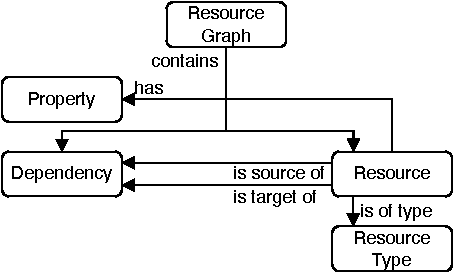
\includegraphics[width=.5\linewidth]{graphics/example.pdf}
  \caption{Example graphics.}
  \label{fig:example}
\end{figure}

And a \Cref{lst:example} \lipsum[6] \Cref{lin:example}

\begin{lstlisting}[
  caption={[Random Stuff.]%
      Random Stuff with a way too long caption.},
  label=lst:example,
  float]
rng.result.apply((wordId) => {
  new aws.s3.BucketObject('index', {
      bucket: bucket, key: 'index.html',
      contentType: 'text/html; charset=utf-8',
      content: '<!DOCTYPE html>' +
               words[wordId].toUpperCase()
  });~\label{lin:example}~
});
\end{lstlisting}

Table stuff going in \Cref{tab:example} \lipsum[6]
\begin{table}
	\caption{Weird table title example.} 
	\label{tab:example}
	\begin{tabular}{lr}
		\toprule
		\multicolumn{2}{c}{Channel \hspace{2cm} Responses} \\ 
		\midrule
		DevOps Chat Slack & 3 \\ 
		Devops Weekly Newsletter & 24  \\ 
		Facebook & 3 \\ 
		LinkedIn & 7 \\ 
		\bottomrule
	\end{tabular}
\end{table}


\section{Publications}
\label{sec:intro:publications}

\newcommand{\ownPub}[1]{\item[\cite{#1}] % get/setmaxcitenames dance ensures that all authors are printed
    \numdef{\origmaxcitenames}{\getmaxcitenames{}}\setmaxcitenames{99}\fullcite{#1}\setmaxcitenames{\origmaxcitenames}}
\newcommand{\ownPubUsed}[2]{\ownPub{#1} \newline [Used in #2]}

This dissertation led to the following publications at peer-reviewed journals, conferences, and workshops.
Their content is used verbatim in this dissertation as stated below.

\begin{itemize}[leftmargin=3em]
    \ownPubUsed{Sokolowski2024Automated}{\Cref{sec:intro}}
\end{itemize}

\noindent
Beyond the publications constituting this dissertation,
I (co)authored the following peer-reviewed articles during my doctoral studies.

\begin{itemize}[leftmargin=3em]
  \ownPub{Sokolowski2024Pipr}
\end{itemize}


% ********************************** Back Matter *******************************
% Backmatter should be commented out, if you are using appendices after References
%\backmatter

%\printglossary[type=\acronymtype]

% ********************************** Bibliography ******************************
\begin{spacing}{0.9}

% To use the conventional natbib style referencing
% Bibliography style previews: http://nodonn.tipido.net/bibstyle.php
% Reference styles: http://sites.stat.psu.edu/~surajit/present/bib.htm

%\bibliographystyle{apalike}
%\bibliographystyle{unsrt} % Use for unsorted references  
%\bibliographystyle{plainnat} % use this to have URLs listed in References
\cleardoublepage

\printbibliography[heading=bibintoc, title={Bibliography}]


\end{spacing}

% ********************************** Appendices ********************************

\begin{appendices} % Using appendices environment for more functunality
    % !TeX spellcheck = en_US
% !TeX encoding = UTF-8
% !TeX root = ../../thesis.tex

\chapter{Nobody Needs This But Your Heart Cannot Get Rid of It}
\label{sec:appA}

\lipsum[1-3]
\end{appendices}

\backmatter

% *************************************** Index ********************************
\printthesisindex % If withindex is present
% !TeX spellcheck = en_US
% !TeX encoding = UTF-8
% !TeX root = thesis.tex

\newcommand{\experienceyearwidth}{1.5cm}
\newcommand{\experiencemonthwidth}{1.1cm}
\newcommand{\experience}[7]{%
    \noindent
	\begin{tabular}{@{} p{\experiencemonthwidth} @{} p{\experienceyearwidth} @{} p{\dimexpr\linewidth - \experienceyearwidth - \experiencemonthwidth\relax} @{}}
		{\leavevmode #1} & {\leavevmode #2} & {\leavevmode #5} \hfill \emph{\leavevmode #6} \\
		{\leavevmode #3} & {\leavevmode #4} & {\leavevmode #7} \\
	\end{tabular}
    \vspace{.3em}
}
\newcommand{\experienceShort}[4]{%
    \noindent
	\begin{tabular}{@{} p{\experiencemonthwidth} @{} p{\experienceyearwidth} @{} p{\dimexpr\linewidth - \experienceyearwidth - \experiencemonthwidth\relax} @{}}
		{\leavevmode #1} & {\leavevmode #2} & {\leavevmode #3} \hfill \emph{\leavevmode #4} \\
	\end{tabular}
    \vspace{-.9em}
}
\newcommand{\teaching}[3]{%
    \noindent
	\begin{tabular}{@{} p{\linewidth} @{}}
		{\leavevmode #1} \hfill \emph{\leavevmode #2} \\
		{\leavevmode #3} \\
	\end{tabular}
    \vspace{.3em}
}

\chapter{Curriculum Vit\ae}

\begin{tabular}{@{} p{\dimexpr \experienceyearwidth + \experiencemonthwidth\relax} @{} l}
    Name & Donald Duck \\
    ORCID & \href{https://orcid.org/...}{...} \\
    Website & \url{https://...} \\
    Citizenship & ...
\end{tabular}

\section*{Education}

\experience
	{Nov.}{2021 --}{June}{2024}
	{Ph.D. in Computer Science}
	{University of St.\,Gallen, Switzerland}
	{Thesis title: Unicorn Dreams.
    Advisor: Prof. Dr. Albert Bob.}

\experienceShort
	{June}{2013}
	{Stuff without second line}
	{Marshmallow, Rainbow}

\section*{Work Experience}

\experience
    {Nov.}{2021 --}{June}{2024}
    {Research Assistant}
    {University of St.\,Gallen, Switzerland}
    {A Group led by Prof. Dr. Albert Bob.}

\section*{Summer Schools}


\section*{Awards}

...

\section*{Service to the Research Community}

\experienceShort{Since}{2020}{Active (shadow) reviewer in %for journals, conferences, and workshops in
the ACM and IEEE Software Engineering and Programming Languages research communities.
\vspace{1em}}{}
    
\experienceShort
    {Oct.}{2023}
    {Student Volunteer at COOLCONF 2023}
    {Cool Place, Great Country}

\section*{Student Supervision}

...

\section*{Teaching Experience}

\teaching
    {Teaching Assistant (exercises, projects, and exams)}
    {University of St.\,Gallen, Switzerland}
    {Lecture: Programming Methodology. \hfill Spring~2023: \textasciitilde30 students.}

\section*{Publications}

The most significant publications so far:

\begin{itemize}[leftmargin=3em]
    \item[\cite{Sokolowski2024Automated}] % get/setmaxcitenames dance ensures that all authors are printed
        \numdef{\origmaxcitenames}{\getmaxcitenames{}}\setmaxcitenames{99}\fullcite{Sokolowski2024Automated}\setmaxcitenames{\origmaxcitenames}
\end{itemize}

\end{document}
